% Options for packages loaded elsewhere
\PassOptionsToPackage{unicode}{hyperref}
\PassOptionsToPackage{hyphens}{url}
%
\documentclass[
]{book}
\usepackage{amsmath,amssymb}
\usepackage{lmodern}
\usepackage{iftex}
\ifPDFTeX
  \usepackage[T1]{fontenc}
  \usepackage[utf8]{inputenc}
  \usepackage{textcomp} % provide euro and other symbols
\else % if luatex or xetex
  \usepackage{unicode-math}
  \defaultfontfeatures{Scale=MatchLowercase}
  \defaultfontfeatures[\rmfamily]{Ligatures=TeX,Scale=1}
\fi
% Use upquote if available, for straight quotes in verbatim environments
\IfFileExists{upquote.sty}{\usepackage{upquote}}{}
\IfFileExists{microtype.sty}{% use microtype if available
  \usepackage[]{microtype}
  \UseMicrotypeSet[protrusion]{basicmath} % disable protrusion for tt fonts
}{}
\makeatletter
\@ifundefined{KOMAClassName}{% if non-KOMA class
  \IfFileExists{parskip.sty}{%
    \usepackage{parskip}
  }{% else
    \setlength{\parindent}{0pt}
    \setlength{\parskip}{6pt plus 2pt minus 1pt}}
}{% if KOMA class
  \KOMAoptions{parskip=half}}
\makeatother
\usepackage{xcolor}
\usepackage{longtable,booktabs,array}
\usepackage{calc} % for calculating minipage widths
% Correct order of tables after \paragraph or \subparagraph
\usepackage{etoolbox}
\makeatletter
\patchcmd\longtable{\par}{\if@noskipsec\mbox{}\fi\par}{}{}
\makeatother
% Allow footnotes in longtable head/foot
\IfFileExists{footnotehyper.sty}{\usepackage{footnotehyper}}{\usepackage{footnote}}
\makesavenoteenv{longtable}
\usepackage{graphicx}
\makeatletter
\def\maxwidth{\ifdim\Gin@nat@width>\linewidth\linewidth\else\Gin@nat@width\fi}
\def\maxheight{\ifdim\Gin@nat@height>\textheight\textheight\else\Gin@nat@height\fi}
\makeatother
% Scale images if necessary, so that they will not overflow the page
% margins by default, and it is still possible to overwrite the defaults
% using explicit options in \includegraphics[width, height, ...]{}
\setkeys{Gin}{width=\maxwidth,height=\maxheight,keepaspectratio}
% Set default figure placement to htbp
\makeatletter
\def\fps@figure{htbp}
\makeatother
\setlength{\emergencystretch}{3em} % prevent overfull lines
\providecommand{\tightlist}{%
  \setlength{\itemsep}{0pt}\setlength{\parskip}{0pt}}
\setcounter{secnumdepth}{5}
\usepackage{booktabs}
\ifLuaTeX
  \usepackage{selnolig}  % disable illegal ligatures
\fi
\usepackage[]{natbib}
\bibliographystyle{plainnat}
\IfFileExists{bookmark.sty}{\usepackage{bookmark}}{\usepackage{hyperref}}
\IfFileExists{xurl.sty}{\usepackage{xurl}}{} % add URL line breaks if available
\urlstyle{same} % disable monospaced font for URLs
\hypersetup{
  pdftitle={FlowMax-Q Manual},
  pdfauthor={Srirama Bhamidipati},
  hidelinks,
  pdfcreator={LaTeX via pandoc}}

\title{FlowMax-Q Manual}
\author{Srirama Bhamidipati}
\date{Last Updated 2024-02-23}

\begin{document}
\maketitle

{
\setcounter{tocdepth}{1}
\tableofcontents
}
\hypertarget{introduction}{%
\chapter{Introduction}\label{introduction}}

\begin{itemize}
\tightlist
\item
  Economy based scenarios are to be modified in the trade-databases.
\item
  Resilience based scenarios (GIS) fall into 2 categories: node-based, edge-based. These in turn fall into 2 categories: editing geometries; editing attributes
\item
  Technology based scenarios will affect the demand (freight composition)
\item
  Policy based scenarios will affect the route and mode choices (freight composition)
\end{itemize}

\hypertarget{introduction-1}{%
\chapter{Introduction}\label{introduction-1}}

\begin{itemize}
\tightlist
\item
  Economy based scenarios are to be modified in the trade-databases.
\item
  Resilience based scenarios (GIS) fall into 2 categories: node-based, edge-based. These in turn fall into 2 categories: editing geometries; editing attributes
\item
  Technology based scenarios will affect the demand (freight composition)
\item
  Policy based scenarios will affect the route and mode choices (freight composition)
\end{itemize}

\hypertarget{scenarios}{%
\chapter{Scenarios}\label{scenarios}}

The image below shows the underlying structure of constructing scenarios

\begin{figure}
\centering
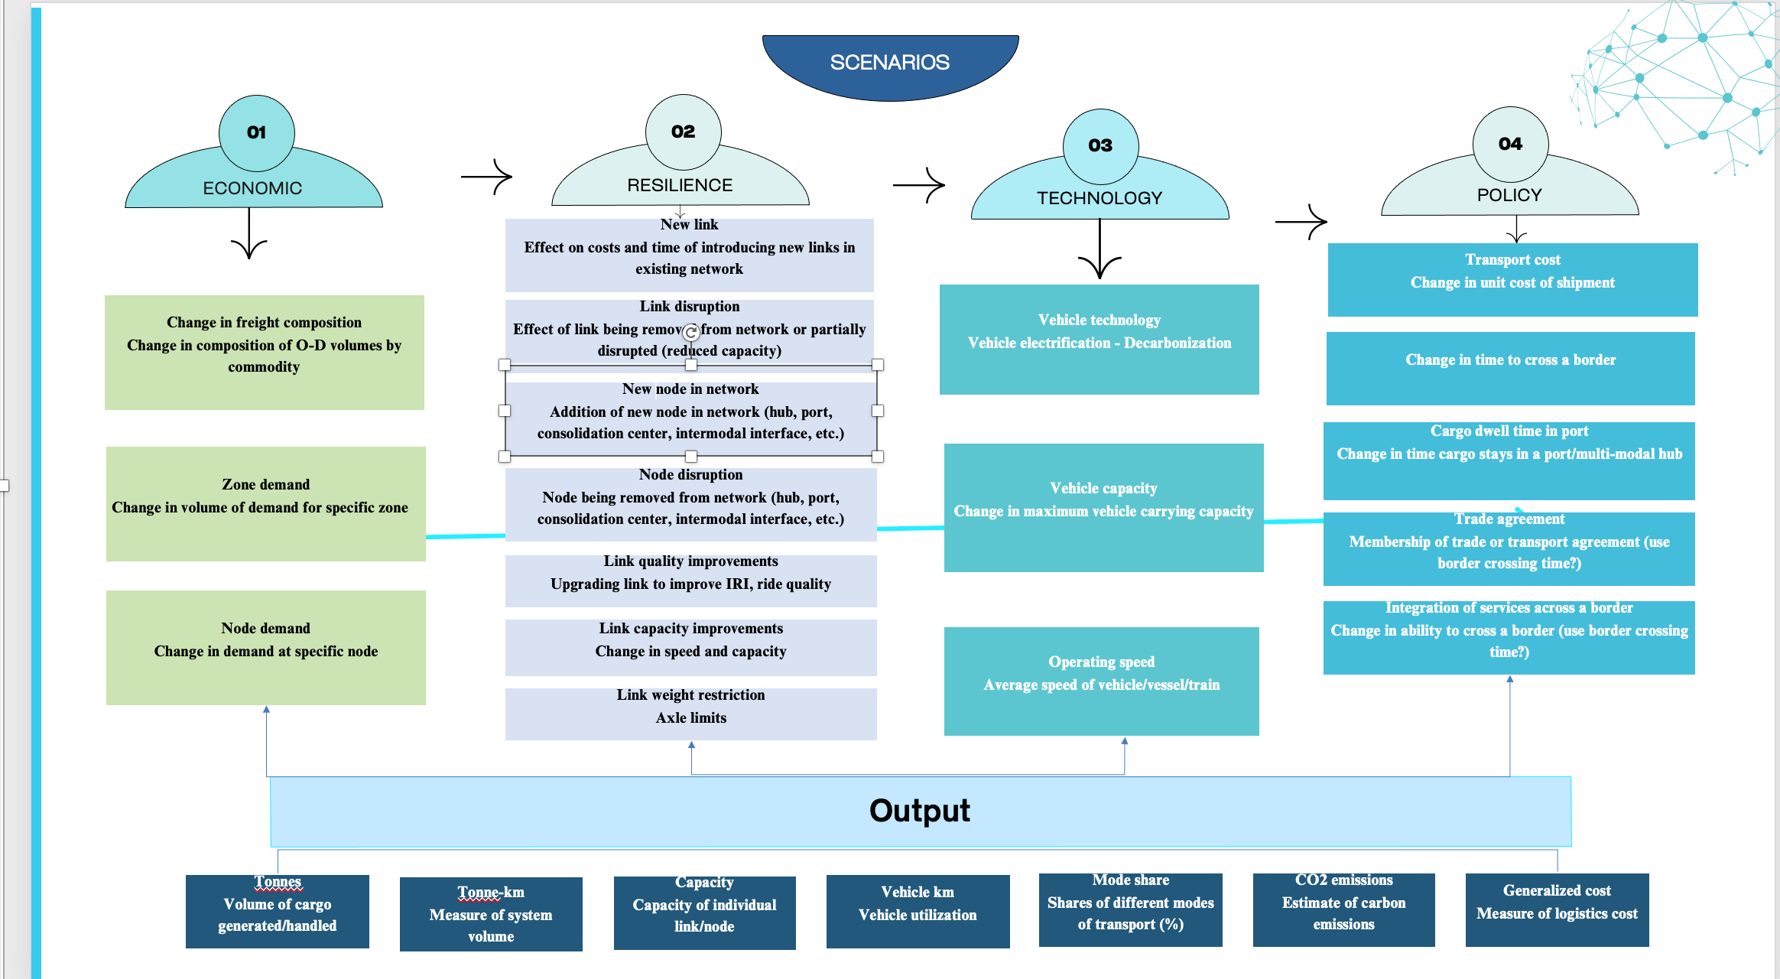
\includegraphics{"./Picture1.png"}
\caption{Scenarios}
\end{figure}

\hypertarget{adding-links}{%
\chapter{Adding Links}\label{adding-links}}

\hypertarget{removing-links}{%
\chapter{Removing Links}\label{removing-links}}

\hypertarget{modifying-node-attributes}{%
\chapter{Modifying Node Attributes}\label{modifying-node-attributes}}

\hypertarget{modifying-edge-attributes}{%
\chapter{Modifying Edge Attributes}\label{modifying-edge-attributes}}

\end{document}
